%章节
%\section{}, \subsection{}, \subsubsection{}, \paragraph{}, \subparagraph{}

%插入图片
%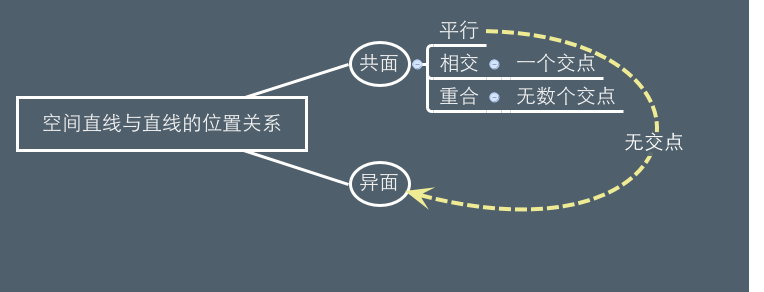
\includegraphics[height=100px]{/Users/shuyue/Desktop/1.png}

%无序列表
%\begin{itemize}
%\item
%\item
%\item
%\item 
%\end{itemize}

%有序列表
%\begin{enumerate}
%\item 
%\item
%\item
%\item
%\end{enumerate}

%嵌套列表
%\begin{itemize}
%\item
%\begin{enumerate}
%\item 
%\item 
%\item 
%\end{enumerate}
%\item
%\begin{enumerate}
%\item 
%\item 
%\item 
%\end{enumerate}
%\end{itemize}

%分栏
%\begin{multicols}{2}
%1\columnbreak \\ 2
%\end{multicols}

%标号
%\textcircled{1}

\documentclass[a4,12pt]{article}
\RequirePackage{CJKutf8,hyperref,mathtools,amssymb,geometry,enumerate,multicol,graphicx,dcolumn}

\begin{document}
\begin{CJK}{UTF8}{gkai}

\title{Solving Irrational Equations}
\date{}
\author{Shuyue Zhang}
\maketitle

\section{教学目标}
\begin{enumerate}
\item 体会无理方程化归为有理方程的过程, 领会其化归思想. 
\item 掌握无理方程的解法.
\item 明白检验的必要性.
\end{enumerate}

\section{教学重点}
\begin{enumerate}
\item 掌握无理方程的解法.
\end{enumerate}

\section{教学难点}
\begin{enumerate}
\item 明白无理方程产生增根的原因.

\end{enumerate}

\section{教学过程}

\subsection{Review}
What kind of equations are called Irrational Equations? Please give an example.\\
Irrational equation is equation, that contains variable under radical.\\
Today we will learn how to solve it.
\subsection{Example 1}
$$x=\sqrt{3x+4}$$\\
Q: How to solve it? You can talk about your thoughts now.\\
Q: Are there any equations that you have learned about their solving?\\
A: Rational equations, including polynomial equations and fractional equations.\vspace{6mm}
\\Square the radical expressions, then the equation will be changed into rational one.\\
Review the property of equation. \\
$p^2=q^2$, if $p=q$.\\
Square both sides,\\
$$x^2=(\sqrt{3x+4})^2.$$
\vspace{6mm}
\\Property:$$(\sqrt{a})^2=a(a \ge 0).$$
So,
$$x^2=3x+4.$$
\\Rewrite it a bit, $$x^2-3x-4=0.$$
\\With Factorization or Quadratic Formula or Vieta Theorem, $$x_1=4, x_2=-1.$$
\vspace{6mm}
\\Q: Does the x here have the same value range with the original one? 
\\Due to the larger range, we may have root not in the initial range. They are extraneous roots.
\\After squaring, there could appear extraneous roots, so we need to check all roots.
\vspace{6mm}
\\Check.
\\Q: How to check?
\\A: Substitute $x=4$ to the both side of the initial equation. Check whether the left equals the right.
\\When $x=4$, $$left=x=4,  right=\sqrt{3x+4}=\sqrt{3\times4+4}=4, left=right.$$
i.e. $x=4$ is a root of the initial equation.
\\When $x= -1$, $$left=x= -1,  right is non-negative, left \neq right.$$
i.e. $x=-1$ is a extraneous root.
\\Therefore, initial equation has only one root: $x=4$.
\\A extraneous root is not a root of the initial equation.

\subsubsection{Key Points}
\begin{enumerate}
\item Isolate the radical expression.
\item Square both sides and simplify.
\item Solve for x.
\item Check for extraneous solutions.
\item Conclusion.
\end{enumerate}

\subsection{Exercise 1}
$$3-\sqrt{2x-3}=x.$$
Rewrite it a bit to leave the radical expression alone on one side,
$$3-x=\sqrt{2x-3}.$$
$$(3-x)^2=(\sqrt{2x-3})^2.$$
With Perfect Square Formula,
$$(a+b)^2=a^2+2ab+b^2.$$
Thus,
\begin{align*}
x^2-6x+9&=2x-3.\\
x^2-8x+12&=0.\\
\end{align*}
$$x_1=2, x_2=6.$$
\\Check.
\\When x=2,
$$left=3-\sqrt{2\times2-3}=2,  right=2, left = right.$$
i.e. $x=2$ is a root of the initial equation.
\\When x=6,
$$left=3-\sqrt{2\times6-3}=0,  right=6, left \neq right.$$
i.e. $x=6$ is a extraneous root.
\\Therefore, initial equation has only one root: $x=2.$

\subsection{Example 2}
\begin{align*}
\sqrt{x}&=\sqrt{3x+4}.\\
x&=3x+4.\\
x&=-2.
\end{align*}
\\Check.
\\When $x=-2$,
$x$ should be non-negative, thus $x=-2$ is a extraneous root.
\\Therefore, initial equation has only no roots.

\subsection{Exercise 2}
\begin{align*}
\sqrt{x^2-2}-\sqrt{2x+1}&=0.\\
\sqrt{x^2-2}&=\sqrt{2x+1}.\\
x^2-2x-3&=0.
\end{align*}
$$x_1=3, x_2=-1.$$
\\Check.
\\When $x=3$,
$$left=\sqrt{7},  right=\sqrt{7}, left= right.$$
i.e. $x=3$ is a root of the initial equation.
\\When $x=-1$, $x^2-2=-1$ is negative.
\\i.e. $x=-1$ is a extraneous root.
\\Therefore, initial equation has only one root: $x=3.$

\subsection{Example 3}
\begin{align*}
\sqrt{x}+2&=\sqrt{3x+4}.\\
x+4\sqrt{x}+4&=3x+4.\\
2\sqrt{x}&=x.\\
4x&=x^2.\\
x^2-4x&=0.
\end{align*}
$$x_1=0, x_2=4.$$
Check.
\\Therefore, initial equation has two roots: $x_1=0, x_2=4.$

\subsection{Exercise 3}
\begin{align*}
\sqrt{x+2}-\sqrt{x}&=1.\\
\sqrt{x+2}&=1+\sqrt{x}.\\
x+2&=1+2\sqrt{x}+x.\\
1&=2\sqrt{x}.\\
x&=\frac{1}{4}.
\end{align*}
Check.
\\Therefore, initial equation has one roots: $x=\frac{1}{4}.$

\subsection{Abstract}
\begin{itemize}
\item After checking, roots may reduce none, part or all.
\item $f(x), g(x), h(x)$ are polynomias.
\begin{enumerate}
\item $\sqrt{f(x)}=g(x).$
\item $\sqrt{f(x)}=\sqrt{g(x)}.$
\item $\sqrt{f(x)}=\sqrt{g(x)}+h(x).$ \\Be changed into No.1 after squaring.
\end{enumerate}
\end{itemize}

\section{Keywords}
\begin{enumerate}
\item Isolate the most complicated radical expression.
\item Square both sides and simplify.
\item Repeat steps 1 and 2 if there was more than one radical expression.
\item Solve for x.
\item Check for extraneous solutions.
\item Conclusion.
\end{enumerate}

\section{Bonus}
$$\sqrt{x+\sqrt{x+11}}+\sqrt{x-\sqrt{x+11}}=4.$$

\end{CJK}
\end{document}